\documentclass{beamer}
\usetheme{Frankfurt}
\usetheme{CambridgeUS}
\usefonttheme{structuresmallcapsserif}
\usefonttheme{serif}
\setbeamertemplate{background canvas}[vertical shading][bottom=white,top=white]   
\setbeamercolor{math text}{fg=black!10!blue}
\setbeamercolor{block title}{bg=blue!40!white, fg=black}
\setbeamertemplate{navigation symbols}{}
\setbeamerfont{frametitle}{size=\normalsize}
\useoutertheme{mathASUlogo}
%\setbeamertemplate{enumerate items}[default]

\usepackage[utf8]{inputenc}
\usepackage[spanish]{babel}
\usepackage{amsmath}
\usepackage{amsfonts}
\usepackage{amssymb}
\usepackage{graphicx}
\usepackage{color}
\usepackage{listings}
\usepackage{hyperref}
\usepackage{wasysym}
\usepackage{alltt}
\usepackage{algorithmic}
\usepackage{cancel}
\usepackage{tikz}
\usetikzlibrary{arrows,backgrounds}
\tikzstyle{block}=[draw opacity=0.7,line width=1.4cm]

\graphicspath{{./Figuras/}{../Figuras/}{./}}
%\graphicspath{{./Figuras/}{../GGMC_2019/Figuras/}}

\definecolor{light-gray}{gray}{0.95}
\definecolor{light-blue}{rgb}{0.90,0.90,0.98}
\definecolor{light-yellow}{rgb}{0.95,0.95,0.10}
\definecolor{dark-green}{rgb}{0.10,0.50,0.10}

\definecolor{links}{rgb}{0.05,0.05,0.95}
\hypersetup{colorlinks,linkcolor=,urlcolor=links}

%%%%%%%%%%%%%%%%%%%%%%%%%%%%%% User specified LaTeX commands.
\newcommand{\Vector}[1]{{\underline{\mathbf{#1}}}}
\newcommand{\Tensor}[1]{{\underline{\underline{\mathbf{#1}}}}}
%%%%%%%%%%%%%%%%%%%%%%%%%%%%%%
% Definimos el punto decimal.
\spanishdecimal{.}
%%%%%%%%%%%%%%%%%%%%%%%%%%%%%%

%Global Background must be put in preamble
%\usebackgroundtemplate%
%{%
%$$\includegraphics[width=0.5\paperwidth]{python-logo}$$%
%}

% the beginning of each subsection:
\AtBeginSection[]
{
	\begin{frame}<beamer>{Contenido}
	\tableofcontents[currentsection]
\end{frame}
}

\title[GeoMaC]{Geof\'isica Matem\'atica y Computacional \\
%\textcolor{Lured}{\footnotesize{... }}\\
%\textcolor{Lured}{\footnotesize{...}}
}   
\author[\copyright LMCS, IGEF--UNAM]{Luis M. de la Cruz Salas} 
\institute[UNAM] 
{ 
{\small{Departamento de Recursos Naturales}} \\
\vspace{0.15cm}
{\small{Instituto de Geof\'isica}} \\ 
\vspace{0.15cm}
{\small{Universidad Nacional Aut\'onoma de M\'exico}} \\
\vspace{0.15cm}

\includegraphics[height=.85cm]{unamlogo.png} 
}

\date{\textcolor{Lured}{\footnotesize{Semestre 2021-I}}}

\subtitle{\textcolor{Lured}{Diferencias Finitas: Problemas No estacionarios}}

% To uncover everything in a step-wise fashion:
%\beamerdefaultoverlayspecification{<+->}


\begin{document}

\begin{frame}
\titlepage
\end{frame}

\begin{frame}{Contenido}
\tableofcontents
\end{frame}

\section{Modelo Matemático: Conducción de calor dependiente del tiempo}

\begin{frame}{}

{\huge MODELO}
$$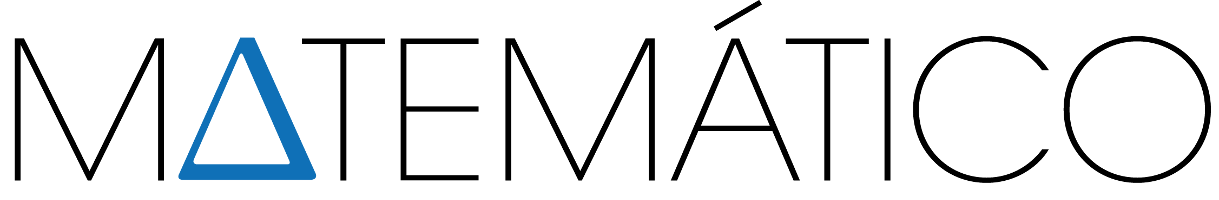
\includegraphics[height=1.5cm]{matematicoCOMPLETO}$$

\end{frame}

\begin{frame}%{Problema no estacionario : Difusi\'on}

Ecuación "general" de transporte de calor (véase \cite{Herrera1}):

\[
c_p \left(\frac{\partial T}{\partial t} + \Vector{v} \cdot \nabla T \right) - \frac{1}{\rho} \nabla \cdot q_x = Q
\]

Usando la ley de Fourier:

\[
c_p \left(\frac{\partial T}{\partial t} + \Vector{v} \cdot \nabla T \right) - \frac{1}{\rho} \nabla \cdot \left(k \nabla T \right) = Q
\]

Conducción de calor NO estacionaria:

\[
\boxed{\frac{\partial T}{\partial t}  + \nabla \cdot \left(k \nabla T \right) = Q}
\]

Cuando $k=constante$:

\[
\boxed{\frac{\partial T}{\partial t}  + k \nabla^2 T = Q}
\]

\end{frame}

\section{Modelo Numérico}

\subsection{Problema de Valor Inicial}

\begin{frame}
\begin{center}
	\fcolorbox{light-gray}{light-gray}{{\Huge \textcolor{black}{Problema de Valor Inicial}}}
\end{center}
\end{frame}

\begin{frame}{Problema no estacionario}
Encontrar $u(x,t)$ que cumpla:
\begin{equation}\label{eq:PVI}
\frac{\partial u}{\partial t} = \frac{\partial}{\partial x} \left( \kappa \frac{\partial u}{\partial x} \right) + Q,
\,\,\, \text{ para } \,\,\, a \leq x \leq b, \,\,\, \text{ y } \,\,\, 0 \leq t \leq T_{max}.
\end{equation}
%
\begin{columns}
\begin{column}{0.40\textwidth}
\begin{description}
	\item[Condiciones iniciales] $u(x,0) = \alpha(x)$

\strut

	\item[Condiciones de frontera]
	$u(a,t)=A(t)$  $u(b,t)=B(t)$
\end{description}
\vspace{2cm}
\end{column}
\begin{column}{0.60\textwidth}
$$\includegraphics[scale=0.45]{df_non_sta_01.pdf}$$
\end{column}
\end{columns}

\end{frame}

\begin{frame}{Problema no estacionario}
$$\includegraphics[scale=0.65]{df_non_sta_02.pdf}$$

\vspace{2cm}

\end{frame}

\begin{frame}{Problema no estacionario}

\[
\frac{\partial u}{\partial t} = \frac{\partial}{\partial x} \left( \kappa \frac{\partial u}{\partial x} \right) + Q,
\,\,\, \text{ para } \,\,\, a \leq x \leq b, \,\,\, \text{ y } \,\,\, 0 \leq t \leq T_{max}.
\]

\begin{itemize}
	\item Cuando $\kappa = constante$, se tiene
	
	\[
	\frac{\partial u}{\partial t} = \kappa \frac{\partial^2 u}{\partial x^2} + Q,
	\,\,\, \text{ para } \,\,\, a \leq x \leq b, \,\,\, \text{ y } \,\,\, 0 \leq t \leq T_{max}.
	\]
	
	\item Si $N_x$ es el n\'umero de inc\'ognitas en $x$, y $N_t$ es el n\'umero de pasos en el tiempo, entonces se definen
	$\displaystyle \Delta x = \frac{b-a}{N_x + 1} = h$ y $\displaystyle \Delta t = \frac{T_{max}}{N_t} = h_t$, como el tama\~no de la malla y el paso de tiempo, respectivamente.
\end{itemize}

\end{frame}


\begin{frame}{Problema no estacionario: semidiscretizaci\'on}

\begin{columns}
	\begin{column}{0.65\textwidth}
		{\small Para cada punto $i$ de la malla espacial podemos aproximar:
			
			$$\left.\dfrac{\partial^2 u}{\partial x^2}\right|_i \approx \dfrac{(u_{i+1} - 2 u_{i} + u_{i-1})}{h^2}$$ 
		}
	\end{column}
	\begin{column}{0.35\textwidth}
		$$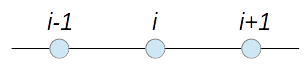
\includegraphics[width = 4cm]{Stencil1D_DF_01}$$
	\end{column}
\end{columns}

Entonces, el problema \eqref{eq:PVI} se transforma en el siguiente Problema de Valor Inicial (PVI):
%
\[
\left.\frac{\partial u}{\partial t}\right|_i = f(t, u_{i+1}, u_{i}, u_{i-1}, Q_i), \,\,\, 0 \leq t \leq T_{max}, \,\,\, \text{ con } u(x_i, 0) = \alpha(x_i)
\]
%
donde $f(t, u_{i+1}, u_{i}, u_{i-1}, Q_i) = \kappa (u_{i+1} - 2 u_{i} + u_{i-1}) / h^2 + Q_i$, para cada $i$ de la malla espacial, junto con las condiciones de frontera correspondientes.

\end{frame}

\subsection{Método de Euler hacia adelante}

\begin{frame}
\begin{center}
	\fcolorbox{light-gray}{light-gray}{{\Huge \textcolor{black}{Método de Euler hacia adelante}}}
\end{center}
\end{frame}

\begin{frame}{Problema no estacionario: Euler hacia adelante (expl\'icito)}

{\small La ecuación
%
\begin{equation}\label{eq:ode01}
\left.\frac{\partial u}{\partial t}\right|_i = f(t, u_{i+1}, u_{i}, u_{i-1}, Q_i)
\end{equation}
%
para $0 \leq t \leq T_{max}$, $i = 1, \dots, N_x$, con condici\'on inicial $u(x_i, 0) = \alpha(x_i) \equiv \alpha_i$ se puede resolver aproximando la derivada temporal usando \textbf{diferencias hacia adelante}:

\begin{equation}\label{eq:ode02}
\left.\frac{\partial u}{\partial t}\right|_i  \approx \frac{u_{i}^{n+1} - u_{i}^{n}}{h_t}
\end{equation}

donde $u_{i}^{n} \equiv u(x_i, t_n)$ y $u_{i}^{n+1} \equiv u(x_i, t_n + h_t)$.

\strut

Sustituyendo \eqref{eq:ode02} en \eqref{eq:ode01} obtenemos:

\begin{equation}\label{eq:EulerAdelante}
\boxed{u_{i}^{n+1} = u_{i}^{n} + h_t \, f(t_n, u_{i+1}^{n}, u_{i}^{n}, u_{i-1}^{n}, Q_i^n)}
\end{equation}

La fórmula \eqref{eq:EulerAdelante} proporciona una forma explícita de encontrar $u_i^{n+1}$ usando valores conocidos del tiempo anterior $n$.
Este es un método \textbf{condicionalmente estable}.

}
\end{frame}

\begin{frame}
\begin{center}
	\fcolorbox{light-gray}{light-gray}{{\Huge \textcolor{black}{Condiciones de frontera:}}}
	\fcolorbox{light-gray}{light-gray}{{\Huge \textcolor{black}{Dirichlet + Dirichlet}}}
\end{center}
\end{frame}

\begin{frame}{Problema no estacionario: Euler hacia adelante (expl\'icito)}

$$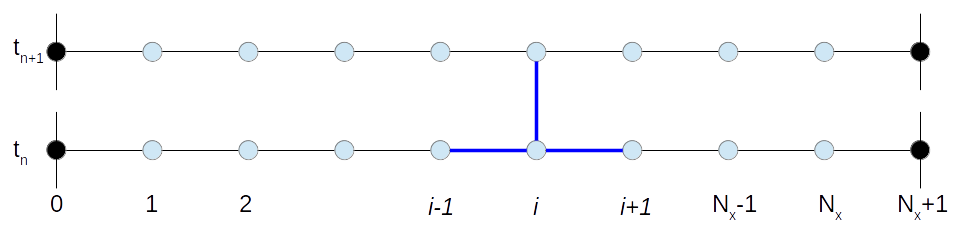
\includegraphics[width=10cm]{Stencil1D_DF_02.png}$$
\begin{footnotesize}
\textbf{Método de Euler hacia adelante} para la ecuación de Poisson: 

\[
\boxed{u_{i}^{n+1} = u_{i}^{n} + r \left(u_{i+1}^{n} - 2 u_{i}^{n} + u_{i-1}^{n}\right) }
\]
%
donde $\displaystyle r = \frac{h_t}{h^2} \kappa$ y suponemos por ahora $Q_i = 0$ para $i=0,\dots,N_x$.

\strut

\textbf{Condiciones de frontera de tipo Dirichlet}: $u_{0}^{n} = A^{n}$ y $u_{N_x+1}^{n} = B^{n}$
\end{footnotesize}
\begin{enumerate}
\item {\footnotesize $u_{1}^{n+1} = u_{1}^{n} + r \left(u_{2}^{n} - 2 u_{1}^{n} + u_{0}^{n}\right) = u_{1}^{n} + r \left(u_{2}^{n} - 2 u_{1}^{n} + \boxed{A^{n}}\right)$}
\item {\footnotesize $u_{N_x}^{n+1} = u_{N_x}^{n} + r \left(u_{N_x+1}^{n} - 2 u_{N_x}^{n} + u_{N_x-1}^{n}\right) = u_{N_x}^{n} + r \left(\boxed{B^{n}} - 2 u_{N_x}^{n} +  u_{N_x-1}^{n} \right)$}
\end{enumerate}

\end{frame}

\begin{frame}{Problema no estacionario: Euler hacia adelante (expl\'icito)}

\begin{footnotesize}
\begin{block}{Algoritmo: Forward Euler (Condiciones de tipo Dirichlet)}
INPUT: $\kappa$, $a$, $b$, $N_x$, $h_t$, $T_{max}$, $A$, $B$, $\alpha_i$ para $i=1,\dots N_x$.

$N_t \leftarrow \text{int}(T_{max} / h_t)$

OUTPUT: $u_i^n$ para $i=1,\dots N_x$ y $ n = 1, \dots, N_t$

\strut
$h \leftarrow (b-a) / (Nx+1)$

$r \leftarrow h_t * \kappa / h^2$

$u_{i}^{0} \leftarrow \alpha_{i}$ para $i=1,\dots N_x$

$u_0^{0} \leftarrow A$

$u_{N_x+1}^0 \leftarrow B$

\strut

DEF $f(r, u_{i+1}^{n}, u_{i}^{n}, u_{i-1}^{n}) : $

$\qquad$ RETURN $r * \left(u_{i+1}^{n} - 2 u_{i}^{n} + u_{i-1}^{n}\right)$

\strut

FOR $ n = 1$ TO $N_t$ DO
\begin{eqnarray*}
u_{i}^{n+1} & \leftarrow & u_{i}^{n} + h_t * f(r, u_{i+1}^{n}, u_{i}^{n}, u_{i-1}^{n}) \text{ para } 
i=1,\dots N_x \\
(\text{plot} & u_i^{n+1} ) \\
u_{i}^{n} & \leftarrow & u_{i}^{n+1}
\end{eqnarray*}
\end{block}
\end{footnotesize}

\end{frame}

\begin{frame}
\begin{center}
	\fcolorbox{light-gray}{light-gray}{{\Huge \textcolor{black}{Condiciones de frontera:}}}
	\fcolorbox{light-gray}{light-gray}{{\Huge \textcolor{black}{Dirichlet + Neumman}}}
\end{center}
\end{frame}

\begin{frame}{Problema no estacionario: Euler hacia adelante (expl\'icito)}

$$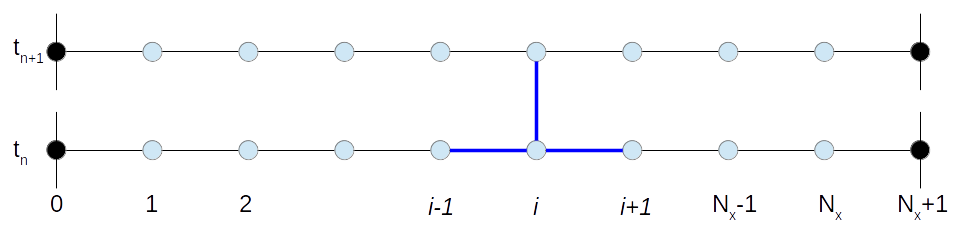
\includegraphics[width=10cm]{Stencil1D_DF_02.png}$$

\begin{footnotesize}
\textbf{Método de Euler hacia adelante} para la ecuación de Poisson: 
%
\[
u_{i}^{n+1} = u_{i}^{n} + r \left(u_{i+1}^{n} - 2 u_{i}^{n} + u_{i-1}^{n}\right) \text{ con } r = \frac{h_t}{h^2} \kappa
\text{ y } Q_i = 0.
\]
%
\textbf{Condiciones de frontera}:
\begin{enumerate}
	\item{\footnotesize  Dirichlet: $u_{0}^{n} = A^{n} \Longrightarrow
	u_{1}^{n+1} = u_{1}^{n} + r \left(u_{2}^{n} - 2 u_{1}^{n} + A^{n}\right)$}
	\item{\footnotesize  Neumman: $\displaystyle \left.\frac{\partial u}{\partial n}\right|_{N_x+1}^{n} = B^{n}
	\Longrightarrow u_{N_x+1}^{n} = h * B^n + u_{N_x}^{n} \qquad $ ($\mathcal{O}(h)$)}
\end{enumerate}
\end{footnotesize}
%
{\footnotesize $ \Rightarrow u_{N_x}^{n+1} = u_{N_x}^{n} + r \left(\boxed{u_{N_x+1}^{n}} - 2 u_{N_x}^{n} + u_{N_x-1}^{n}\right) = 
	u_{N_x}^{n} + r  \left(h * B^{n} - u_{N_x}^{n} +  u_{N_x-1}^{n} \right)$}

\end{frame}

\begin{frame}{Problema no estacionario: Euler hacia adelante (expl\'icito)}

\begin{footnotesize}

\begin{block}{Algoritmo: Forward Euler (Cond. Dirichlet + Neumman)}
INPUT: $\kappa$, $a$, $b$, $N_x$, $h_t$, $T_{max}$, $A$, $B$, $\alpha_i$ para $i=1,\dots N_x$.

$N_t = \text{int}(T_{max} / h_t)$

OUTPUT: $u_i^n$ para $i=1,\dots N_x$ y $ n = 1, \dots, N_t$

\strut
$h = (b-a) / (Nx+1)$

$r = h_t * \kappa / h^2$

$u_{i}^{0} \leftarrow \alpha_{i}$ para $i=1,\dots N_x$

$u_0^{0} \leftarrow A$

\strut

DEF $f(r, u_{i+1}^{n}, u_{i}^{n}, u_{i-1}^{n}) : $

$\qquad$ RETURN $r * \left(u_{i+1}^{n} - 2 u_{i}^{n} + u_{i-1}^{n}\right)$

\strut

FOR $ n = 1$ TO $N_t$ DO
\begin{eqnarray*}
u_{N_x+1}^n & \leftarrow & h * B^n + u_{N_x}^n \\
u_{i}^{n+1} & \leftarrow & u_{i}^{n} + h_t * f(r, u_{i+1}^{n}, u_{i}^{n}, u_{i-1}^{n}) \text{ para } 
i=1,\dots N_x \\
(\text{plot} & u_i^{n+1}) \\
u_{i}^{n} & \leftarrow & u_{i}^{n+1}
\end{eqnarray*}
\end{block}
\end{footnotesize}

\end{frame}

\subsection{Método de Euler hacia atrás}

\begin{frame}
\begin{center}
	\fcolorbox{light-gray}{light-gray}{{\Huge \textcolor{black}{Método de Euler hacia atrás}}}
\end{center}
\end{frame}

\begin{frame}{Problema no estacionario: Euler hacia atr\'as (impl\'icito)}

La ecuación
\begin{equation}\label{eq:ode03}
\left.\frac{\partial u}{\partial t}\right|_i = f(t, u_{i+1}, u_{i}, u_{i-1}, Q_i)
\end{equation}
para $0 \leq t \leq T_{max}$, $i=0,\dots,N_x$ ,con condici\'on inicial $u(x_i, 0) = \alpha(x_i) \equiv \alpha_i$ se puede 
resolver aproximando la derivada temporal usando \textbf{diferencias hacia atrás}:
%
\begin{equation}\label{eq:ode04}
\left.\frac{\partial u}{\partial t}\right|_i  \approx \frac{u_{i}^{n} - u_{i}^{n-1}}{h_t}
\end{equation}

donde $u_{i}^{n} \equiv u(x_i, t_n)$ y $u_{i}^{n-1} \equiv u(x_i, t_n - h_t)$. 

\strut

Sustituyendo \eqref{eq:ode04} en \eqref{eq:ode03} obtenemos:

\[
\boxed{u_{i}^{n} = u_{i}^{n-1} + h_t \, f(t_n, u_{i+1}^{n}, u_{i}^{n}, u_{i-1}^{n}, Q_i^n)}
\]
%
\end{frame}


\begin{frame}{Problema no estacionario: Euler hacia atr\'as (impl\'icito)}

$$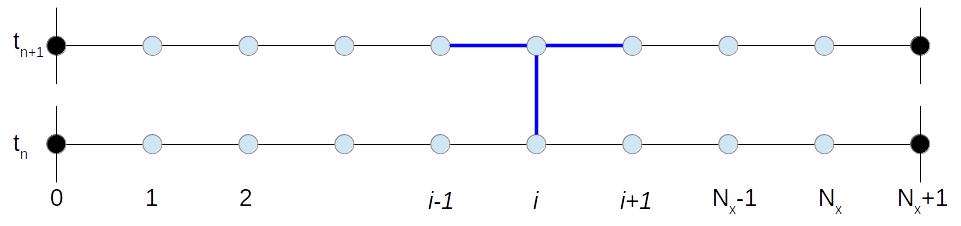
\includegraphics[width=10cm]{Stencil1D_DF_03.png}$$

\begin{footnotesize}
\textbf{Método de Euler hacia atrás} para la ecuación de Poisson: 

\begin{equation} \label{eq:EulerAtras}
\boxed{u_{i}^{n} = u_{i}^{n-1} + r \left(u_{i+1}^{n} - 2 u_{i}^{n} + u_{i-1}^{n}\right) }
\end{equation}
%
donde $\displaystyle r = \frac{h_t}{h^2} \kappa$ y suponemos por ahora $Q_i = 0$ para $i=0,\dots,N_x$.

\strut

En la f\'ormula \eqref{eq:EulerAtras} observamos que tenemos tres incógnitas $u_{i}^n$, $u_{i+1}^n$ y $u_{i-1}^n$; y un valor conocido en el tiempo anterior $u_{i}^{n-1}$. Por lo tanto la fórmula es impl\'icita y se debe resolver un sistema de ecuaciones. Este método es \textbf{incondicionalmente estable}.
\end{footnotesize}

\end{frame}

\begin{frame}{Problema no estacionario: Euler hacia atr\'as (impl\'icito)}

Este método genera el siguiente sistema de ecuaciones
\begin{eqnarray*}
u_{1}^{n} & = & u_{1}^{n-1} + r \left(u_{2}^{n} - 2 u_{1}^{n} + \boxed{u_{0}^{n}}\right) \,\,\, \mbox{ Cond. de frontera}\\
u_{2}^{n} & = & u_{2}^{n-1} + r \left(u_{3}^{n} - 2 u_{2}^{n} + u_{1}^{n}\right) \\
\dots & \dots & \dots \\
u_{i}^{n} & = & u_{i}^{n-1} + r \left(u_{i+1}^{n} - 2 u_{i}^{n} + u_{i-1}^{n}\right) \\
\dots & \dots & \dots \\
u_{N_x}^{n} & = & u_{N_x}^{n-1} + r \left(\boxed{u_{N_x+1}^{n}} - 2 u_{N_x}^{n} + u_{N_x-1}^{n}\right) \,\,\, \mbox{ Cond. de frontera}\\
\end{eqnarray*}
%
Condiciones de frontera:
\begin{eqnarray*}
u_{1}^{n} & = & u_{1}^{n-1} + r \left(u_{2}^{n} - 2 u_{1}^{n} + \boxed{A^{n}}\right) \,\,\,\,\, \mbox{(Dirichlet)} \\
u_{N_x}^{n} & = & u_{N_x}^{n-1} + r \left(\boxed{h B^{n} + u_{N_x}^{n}} - 2 u_{N_x}^{n} + u_{N_x-1}^{n}\right) \,\,\,\,\, \mbox{(Neumman)}\\
\end{eqnarray*}

\end{frame}

\begin{frame}{Problema no estacionario: Euler hacia atr\'as (impl\'icito)}

\begin{footnotesize}
Escribimos el sistema de ecuaciones anterior como sigue:

\begin{eqnarray*}
-r u_{2}^{n} + (1+2r) u_{1}^{n} & = & u_{1}^{n-1} + r A^{n}\\
-r u_{3}^{n} + (1+2r) u_{2}^{n} - r u_{1}^{n} & = & u_{2}^{n-1} \\
\dots & \dots & \dots \\
-r u_{i+1}^{n} + (1+2r) u_{i}^{n} - r u_{i-1}^{n} & = & u_{i}^{n-1} \\
\dots & \dots & \dots \\
(1+r) u_{N_x}^{n} - r u_{N_x-1}^{n} & = & u_{N_x}^{n-1} + r h B^{n}\\
\end{eqnarray*}
%
En forma matricial:
\[
\left[
\begin{matrix}
(1+2r) & -r     & 0      & 0      & 0      & 0  \\
-r     & (1+2r) & -r     & 0      & 0      & 0  \\
0      & -r     & (1+2r) & -r     & 0      & 0  \\
0      & 0      & -r     & (1+2r) & -r     & 0  \\
\vdots & \vdots & \vdots & \vdots & \ddots & \vdots \\
0      & 0      & 0      & 0      & -r     & (1+r) 
\end{matrix}
\right] \left[
\begin{matrix}
u_{1}^{n} \\ u_{2}^{n} \\u_{3}^{n} \\u_{4}^{n} \\ \vdots \\u_{N_x}^{n}
\end{matrix}
\right] = \left[
\begin{matrix}
u_{1}^{n-1} + rA^{n} \\ u_{2}^{n-1} \\u_{3}^{n-1} \\u_{4}^{n-1} \\ \vdots \\u_{N_x}^{n-1} + rh B^{n}
\end{matrix}
\right]
\]
\end{footnotesize}

\end{frame}

\subsection{Convergencia, Consistencia, Estabilidad}

\begin{frame}
\begin{center}
	\fcolorbox{light-gray}{light-gray}{{\Huge \textcolor{black}{Convergencia, consistencia y}}}
	\fcolorbox{light-gray}{light-gray}{{\Huge \textcolor{black}{estabilidad}}}
\end{center}
\end{frame}

\begin{frame}{Estabilidad: Euler Forward vs. Euler Backward}

\begin{small}

\begin{columns}
\begin{column}{0.45\textwidth}
\textbf{Euler Forward (Expl\'icito)}

\begin{itemize}
\item La evaluaci\'on de $u_i^{n+1}$ se realiza mediante la evaluaci\'on de una f\'ormula expl\'icita.
\item Cada una de estas evaluaciones es independiente de las otras, por lo que este esquema es paralelizable directamente.
\item Es condicionalmente estable: $\frac{h_t}{h^2} \kappa < \frac{1}{2} \Longrightarrow h_t < \frac{h^2}{2 \kappa}$.
\item La condici\'on anterior obliga a realizar muchos pasos de tiempo para llegar a $T_{max}$.
\end{itemize}
\end{column}
\begin{column}{0.45\textwidth}
\textbf{Euler Backward (Impl\'icito)}
\begin{itemize}
\item La soluci\'on en el paso $n+1$ se encuentra resolviendo un sistema lineal de ecuaciones.
\item Es posible paralelizar la soluci\'on del sistema lineal.
\item Es incondicionalmente estable, por lo que $h_t$ puede ser grande.
\item Si la matriz del sistema est\'a mal condicionada, la soluci\'on de un paso de tiempo puede tardar mucho.
\end{itemize}
\end{column}
\end{columns}

\begin{itemize}
\item En ambos casos el orden de la aproximaci\'on es $\mathcal{O}(h^2) + \mathcal{O}(h_t)$.
\end{itemize}
\end{small}

\end{frame}

\begin{frame}{Convergencia, consistencia y estabilidad}
\begin{itemize}
\item \textbf{Convergencia} : 
Es la propiedad de un m\'etodo num\'erico de producir una soluci\'on 
que aproxima a la soluci\'on exacta conforme la distancia entre los 
puntos de la malla tiende a cero. 
\item \textbf{Consistencia} :
Un esquema num\'erico consistente produce sistemas de ecuaciones 
algebraicas equivalentes a las ecuaciones gobernantes originales 
cuando el espaciamiento de los nodos de la malla tiende a cero. 
\item \textbf{Estabilidad} ;
La estabilidad est\'a asociada con la amortiguaci\'on del error 
conforme el m\'etodo num\'erico procede. 
\end{itemize}

\begin{block}{Teorema de equivalencia de Lax}
Para problemas lineales una condici\'on necesaria y suficiente 
para obtener convergencia es que el m\'etodo sea consistente y estable. 
\end{block}

\end{frame}

\subsection{Esquema Crank-Nicholson}

\begin{frame}
\begin{center}
	\fcolorbox{light-gray}{light-gray}{{\Huge \textcolor{black}{Esquema Crank-Nicholson}}}
\end{center}
\end{frame}

\begin{frame}{Problema no estacionario: Crank-Nicholson (impl\'icito)}

$$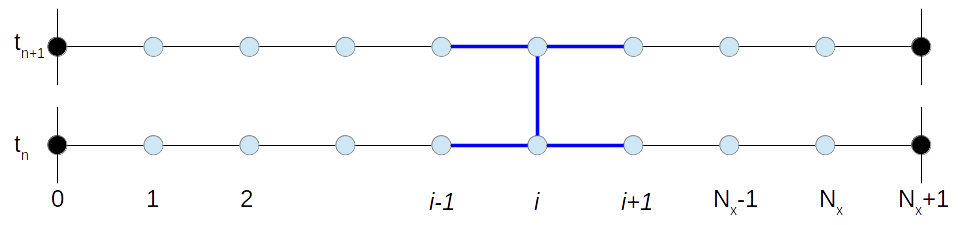
\includegraphics[width=10cm]{Stencil1D_DF_04.png}$$

\begin{footnotesize}

Esquema con la propiedad  en $\mathcal{O}(h^2 + h_t^2)$. Aproximamos en $(x_i,t^{n+\frac{1}{2}})$:
\begin{eqnarray*}
\left.\dfrac{\partial u}{\partial t}\right|_{i}^{n+\frac{1}{2}} & = & \dfrac{u_{i}^{n+1} - u_i^{n}}{h_t} \\ 	
\left.\dfrac{\partial^2 u}{\partial x^2}\right|_{i}^{n+\frac{1}{2}} & = & 
\frac{\kappa}{2} 
\left[  
\frac{\left(u_{i+1}^{n+1} - 2 u_{i}^{n+1} + u_{i-1}^{n+1}\right)}{h^2} + 
\frac{\left(u_{i+1}^{n} - 2 u_{i}^{n} + u_{i-1}^{n}\right)}{h^2}
\right]
\end{eqnarray*}	
\textbf{Método de Crank-Nicholson}:
\begin{equation}\label{eq:CrankNicholson}
\boxed{u_{i}^{n+1} -  \frac{r}{2} \left(u_{i+1}^{n+1} - 2 u_{i}^{n+1} + 
u_{i-1}^{n+1}\right) = u_{i}^{n} + \frac{r}{2} \left(u_{i+1}^{n} - 2 u_{i}^{n} + u_{i-1}^{n}\right)}
\end{equation}
La f\'ormula \eqref{eq:CrankNicholson} es impl\'icita y condicionalmente estable.

\end{footnotesize}

\end{frame}

%\section{Modelo Computacional}
%
%\begin{frame}{Lista de cotejo}
%
%\begin{itemize}
%	\item Método de Euler hacia adelante
%	\item Método de Euler hacia atrás
%	\item Método de Crank-Nicholson	
%\end{itemize}
%
%\end{frame}
%
%\subsection{Calibración}
%
%\begin{frame}
%\begin{center}
%	\fcolorbox{light-gray}{light-gray}{{\Huge \textcolor{black}{Calibración}}}
%\end{center}
%\end{frame}
%
%\begin{frame}{Ecuaci\'on de calor en 2D}
%
%\begin{columns}
%	\begin{column}{0.3\textwidth}
%		$$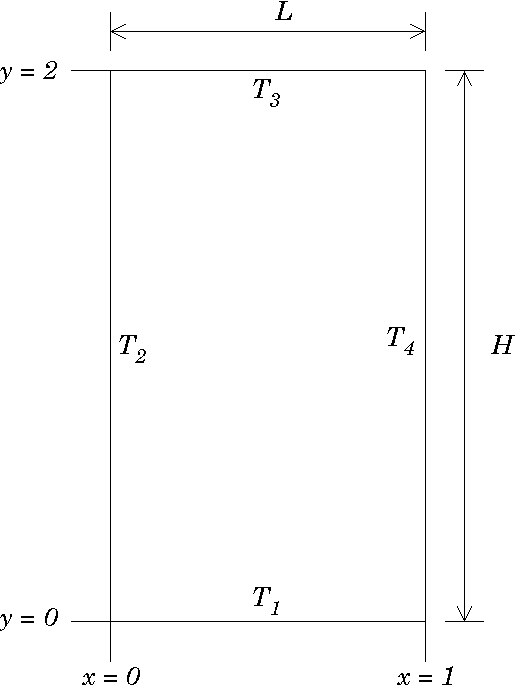
\includegraphics[width=2.5cm]{Hoffman.png}$$
%	\end{column}
%	\begin{column}{0.3\textwidth}
%		$$\includegraphics[width=2.5cm]{HoffmanExact.png}$$
%	\end{column}
%	\begin{column}{0.3\textwidth}
%		$$\includegraphics[width=3cm]{HoffmanExactS.png}$$
%	\end{column}
%\end{columns}
%
%{\footnotesize{
%		\begin{itemize}
%			\item Ecuaci\'on y condiciones iniciales y de frontera
%			\begin{eqnarray*}
%				\frac{\partial T(\Vector{x},t)}{\partial t} & = & \nabla^2 T(\Vector{x}, t) \,\,\,\,\, \text{para} \,\,\,\,\, \Vector{x} \in [0,1] \times [0,2]  \,\,\, \text{y} \,\,\, 0 \leq t \leq T_{max} \\
%				T_1 & = & 100; T_2 = T_3 = T_4 = 0 \,\,\,\,\, \text{(Cond. de frontera)} \\
%				T(\Vector{x}, 0) & = & 0 \,\,\,\,\, \text{para} \,\,\,\,\, \Vector{x} \in (0,1) \times (0,2) \,\,\, \text{(Cond. inicial)} 
%			\end{eqnarray*}
%			\item Soluci\'on exacta: similar a la soluci\'on del caso estacionario cuando $t \rightarrow \infty$.
%			
%		\end{itemize}
%}}
%
%\end{frame}

\section<presentation>{Referencias}

\begin{frame}[allowframebreaks]
	%\frametitle<presentation>{Bibliograf\'{\i}a}
	
\begin{thebibliography}{10}
		
{\footnotesize 

% BOOKS 
\beamertemplatebookbibitems


\bibitem{Leveque}
[1] R.J. Leveque,
\newblock {\em Finite Difference Method for Ordinary and Partial Differential Equations: Steady State and Time-Dependent Problems },
\newblock {Society for Industrial and Applied Mathematics (SIAM), Philadelphia}, \textbf{2007}.

\bibitem{Saad}
[2] Y. Saad
\newblock {\em Iterative Methods for Sparse Linear Systems}.
\newblock PWS/ITP 1996.
\newblock {Online: 
	\textsf{http://www-users.cs.umn.edu/\textasciitilde saad/books.html}, 
	\textbf{2000}}

\bibitem{Burden}
[3]  Richard Burden and J. Douglas Faires
\newblock{\em Numerical Analysis}
\newblock Cengage Learning; 9 edition (August 9, \textbf{2010})

\bibitem{Herrera1} 
[4] I. Herrera \& G. F. Pinder,
\newblock {\em Mathematical Modeling in Science and Engineering: An Axiomatic Approach}, 
\newblock John Wiley \textbf{2012}.

% ARTICULOS    
\beamertemplatearticlebibitems

%\bibitem{Delacruz2011}
%[7]   L. M. de la Cruz,
%\newblock Flujo en una y dos fases en medios porosos: modelos matemáticos, numáricos y computacionales,
%\newblock {\em Reportes técnicos del Instituto de Geofísica}, 2012-4, Agosto \textbf{2012}.


}
		
\end{thebibliography}
\end{frame}

\end{document}
	